% You should title the file with a .tex extension (hw1.tex, for example)
\documentclass[a4paper, 11pt]{article}

\usepackage{amsmath}
\usepackage{amssymb}
\usepackage{fancyhdr}
\usepackage{tikz}

\usepackage[margin=1in]{geometry}

\newcommand{\question}[2] {\vspace{.25in} \hrule\vspace{0.5em}
\noindent{\bf #1: #2} \vspace{0.5em}
\hrule \vspace{.10in}}
\renewcommand{\part}[1] {\vspace{.10in} {\bf (#1)}}

\newcommand{\myname}{Poonnarat Nakartit}
\newcommand{\myemail}{poonpptn@gmail.com}
\newcommand{\myhwnum}{homework-number-3}

\setlength{\parindent}{0pt}
\setlength{\parskip}{5pt plus 1pt}
 
\pagestyle{fancyplain}
\lhead{\fancyplain{}{\textbf{HW\myhwnum}}}      % Note the different brackets!
\rhead{\fancyplain{}{\myname\\ \myemail}}
\chead{\fancyplain{}{ICCS200 }}

\begin{document}

\medskip                        % Skip a "medium" amount of space
                                % (latex determines what medium is)
                                % Also try: \bigskip, \littleskip

\thispagestyle{plain}
\begin{center}                  % Center the following lines
{\Large ICCS200: Assignment \myhwnum } \\
\myname  \
\myemail \\
Recitation: Your recitation section \\
The date \\
\end{center}

\question{Exercise 1}{Tail Sum of Squares (2 points)}
\begin{verbatim}
int sumHelper(int n , int a) {
	if (n==0) return a;
	else returnsumHelper(n-1,a+n*n);
}
int sumSqr(int n) { return sumHelper(n, 0); }
\end{verbatim}
\\
Prove that for $n\geq1$, \texttt{sumSqr(n)}  is $1^{2}+2^{2}+3^{2}+...+n^{2}$. To prove this, use induction to show that \texttt{sumHelper} computes the "right thing".
\begin{itemize}
\item Predicate: P(n):= $\forall n $ and $\forall a \in \mathbb{I^{+}}$+set of zero and $n>0$ \texttt{sumhelper(int n, int a)} returns $1^{2} + 2^{2} +3^{2}+...+n^{2} + a$ .\\
\item Base case: P(0)  \texttt{sumhelper(0, int a)} returns a
\item Inductive step:  Assume that $\forall k \leq n$ where $k \in \mathbb{I^{+}}$ \texttt{sumhelper(int , int a)} returns 
$1^{2} + 2^{2} +3^{2}+...+k^{2} + a$ .\\
Want to show that \texttt{sumhelper(k+1,a')} returns $1^{2} + 2^{2} +3^{2}+...+k^{2} + a +(k+1)^{2} + a'$.\\
\\ 
Since $k+1 > 0$  \texttt{sumhelper(k+1,a')} return \texttt{sumhelper(k,a)} returns \texttt{sumhelper(k, a'+ (k+1)*(k+1))}.\\
Because of we know that \texttt{sumhelper(k, a)} returns $1^{2} + 2^{2} +3^{2}+...+k^{2} + a +(k+1)^{2} + a$. Where a is equal to \texttt{a'+ (k+1)*(k+1)} ,so $1^{2} + 2^{2} +3^{2}+...+k^{2} + a +(k+1)^{2} + a'$ by inductive hypothesis.  And we have just established that for $n > 0$, if P(k) is true, then P(k+1)is true.
\end{itemize}

\question{Exercise 2}{Mysterious Function (2 points)}
\begin{itemize}
\item Predicate: P(n) := $n \geq1$, if \texttt{foo(n) returns (p, q)}, then 
\begin{eqnarray*}
			  \frac{p}{q} &=& \frac{n}{n+1}
\end{eqnarray*}
\item Base case: P(1) = \text{foo(1) returns (1,2)}, so $\frac{1}{2} = \frac{1}{1+1} $\\
\\
\item Inductive step: Assume that$\forall k < =n$. P(k)= \texttt{foo(k) returns (p,q), which is equal to $\frac{p}{q} =\frac{n}{n+1}$ }
\\
Want to show that P(k+1) = \texttt{foo(k+1)} = $\frac{p'}{q'} = \frac{k+1}{k+2}$
\\
\\
Since the k +1 is more than 1, the algorithm returns \texttt{foo(k)}, which is the inductive hypothesis. We will get $\frac{p}{q} =\frac{n}{n+1}$, and \text{foo(k+1 ) returns (p',q')}, which p' is equal to $(k+1)+k*(k+1)*(k+2)$, and q' is equal to $(k+1)*(k+1)*(k+2)$
\\
\\
Want to show that :  $\frac{p'}{q'} == \frac{k+1}{k+2}$
\begin{eqnarray*}
	\frac{p'}{q'} &=& \frac{(k+1)+k*(k+1)*(k+2)}{(k+1)*(k+1)*(k+2)}\\
	&=& \frac{k+1}{(k+1)*(k+1)*(k+2)} + \frac{k*k+1*k+2}{(k+1)*(k+1)*(k+2)}\\
	&=&	\frac{1}{(k+1)(k+2)} + \frac{k}{k+1}\\
	&=&\frac{k(k+2)+1}{(k+1)(k+2)}\\
	&=&\frac{k^{2}+2k+1}{(k+1)(k+2)}\\
	&=&\frac{(k+1)(k+1)}{(k+1)(k+2)}
	&=&\frac{p'}{q'}
	&=&\frac{k+1}{k+2}\\
\end{eqnarray*}
By mathematical induction,  $n \geq1$, if \texttt{foo(n) returns (p, q)}, then 
\begin{eqnarray*}
	\frac{p}{q} &=& \frac{n}{n+1}
\end{eqnarray*} is true.
\end{itemize}
\question{Exercise 3}{Missing Tile (4 points)}
Task I: We know you’ve seen this proof already. But so that you fully understand how it works, you’ll prove this theorem again, in your own words, by induction on n.
\begin{itemize}
	\item Predicate: P(n):= Any where$b \leq 2$. $2^{n} -by-2{n}$ grid with one painted cell can be tiled using $L-shaped$ triominoes
such that the entire grid is covered by triominoes but no triominoes overlap with each other
nor the painted cell.
	\item Base cases: P(2):= \begin{figure}[!htbp]
		\begin{center}
			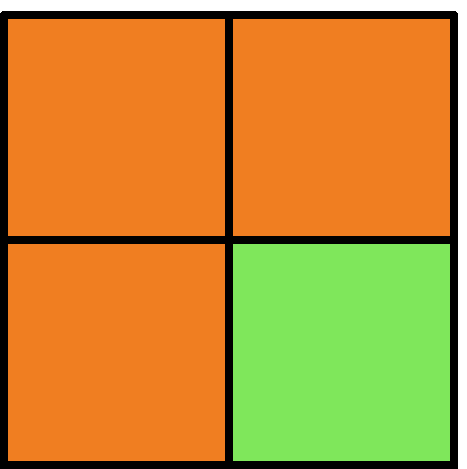
\includegraphics [width=2cm]{data1.png}
		\end{center}
		\caption{The green color is the painted grid, orenge is the l-shape. The other basecases are just the oreantation of this figure}\label{lines}
	\end{figure}
	\item Inductive step: = Assume that $\forall k \leq n$ P(k):= Any where$b \leq 2$. $2^{k} -by-2{k}$ grid with one painted cell can be tiled using $L-shaped$ triominoes
	such that the entire grid is covered by triominoes but no triominoes overlap with each other
	nor the painted cell. 
	\\
	Want to show that: P(k+1):= $2^{k+1} -by-2{k+1}$ grid with one painted cell can be tiled using $L-shaped$ triominoes
	such that the entire grid is covered by triominoes but no triominoes overlap with each other
	nor the painted cell. 
	\\
	This $2^{k+1}-by-2^{k+1}$ can be break down into four pieces of size $2\times2^{k}$
	\begin{eqnarray*}
		2^{2+1} \times 2^{2+1} &=& \\
		2^2\times2^{k}\times2^{k}
		&=& 4\times2^{k}\times 2^{k}
	\end{eqnarray*} 
	Since we know that 2^{k} is hold by inductive hypothesis.
	By matematical induction, Any where$b \leq 2$. $2^{n} -by-2{n}$ grid with one painted cell can be tiled using $L-shaped$ triominoes such that the entire grid is covered by triominoes but no triominoes overlap with each other
	nor the painted cell.
	
\end{itemize}





\question{Exercise 5}{Midway Tower of Hanoi (6 points)}
Task II: Solve the following inputs by hand. They are presented in the same format as described above. Document the reasoning you use to reach the answers. You want a process that will work with larger inputs.

\item $\{2, 2, 1\}\to\{0, 2, 1\}\to\{0, 1, 1\}\to\{1, 1, 1\}$\\
\item$\{2, 1, 0\}\to\{0, 1, 0\}\to\{0, 2, 0\}\to\{2, 2, 0\}\to\{2, 2, 1\}\to\{0, 2, 1\}\to\{0, 1, 1\}\to\{1, 1, 1\}$\\

My Logic is just trying to move the bigest disk in place to do that, I need to move the smaller $n-1$ disks first, which It is $2^{n-1} -1$ moves. so I can move the biggest one in place,add $1$ move, and moves the others back to the destination peg using $2^{n-1} -1$ moves.
\\
\\
Task III: Prove, using induction, that for any $n \geq 0 $, \texttt{solve$\_$hanoi(n, ...)}generates exactly $2^{n} -1$ lines of instructions.

\begin{verbatim}
def solve_hanoi(n, from_peg, to_peg, aux_peg): 
       if n>0:
           solve_hanoi(n-1, from_peg, aux_peg, to_peg)
           print "Move disk", n-1, "from Peg", from_peg, "to Peg", to_peg
           solve_hanoi(n-1, aux_peg, to_peg, from_peg)
solve_hanoi(n, 0, 1, 2)

\end{verbatim}

\begin{itemize}
	\item Predicate: P(n):= \texttt{solve\_hano(n, from\_peg, to\_peg, aux\_peg)} use $2^{n}-1$ lines of instructions.
	\item P(1):= \texttt{solve\_hano(1, from\_peg, to\_peg, aux\_peg)} use $2^{1}-1 = 1$ 
	\item Inductive step: Assume that  $ \forall k < =n$ P(k):= \texttt{solve\_hano(k, from\_peg, to\_peg, aux\_peg)} use $2^{k}-1$ lines of instructions.
	\\ Want to show that P(k+1):= \texttt{solve\_hano(k+1, from\_peg, to\_peg, aux\_peg)} use $2^{k+1}-1$ lines of instructions.
	\\
	In the first recursive call, \texttt{solve\_hano(k, from\_peg, to\_peg, aux\_peg)} performs $2^{k-1}$ lines of instructions as well as the second the second call by inductive hypothesis. and perfrom one line of instruction on the print stagement.
	\begin{eqnarray*}
	(2^{k} -1) + 1 + (2^{k} -1) = 2*2^{k} -1 = 2^{k+1} -1
	\end{eqnarray*}
	by mathematical induction texttt{solve\_hano(n, from\_peg, to\_peg, aux\_peg)} use $2^{n}-1$ lines of instructions.
	P(1):= \texttt{solve\_hano(1, from\_peg, to\_peg, aux\_peg)} use $2^{1}-1 = 1$ is true.
\end{itemize}



\end{document}

